\documentclass[11pt]{article}
\usepackage{mypackages}
\begin{document}

\subsection{Improving policies}

Now that we can update and maintain an estimator of the value function, we want
to focus on improving our policy.
As something new, we learn the policy as a parameterized function $\pi(a, s, \theta_t)$
, which given an action $a$ and a state $s$ returns the probability
of taking action $a$ in state $s$ using the weights $\theta_t$.
The goal of the learning agent is to find the best policy, which is the one 
that will maximize the expected return.
To examine how well a policy is doing, we use a \textit{performance measure}, $\rho(\theta_t)$, to evaluate
the policy based on the policy weights $\theta_t$.
We want to maximize the performance measure, since the policy is then optimal with
respects to $\rho(\theta_t)$.
Like in section \ref{sec:td}
we perform gradient ascent to find the optimal weights of the performance measure,
and thus, the update of the policy weights is defined as
\begin{equation}
    \theta_{t+1} = \theta_t + \alpha \nabla_{\theta_t} \rho(\theta_t)
\end{equation}
where $\alpha$ is a parameter determining the step size of the gradient ascent.

We want the performance measure to favor actions that are rarely taken, so that
their contribution to the weights are the same as the actions that are
picked more often.
This means that a larger gradient step should be performed if there is a small probaility
of sampling the action and the following performance measure can be constructed
\begin{equation}
    \begin{aligned}
        \rho(\theta_t) & = \log\pi(a|s, \theta_t)
    \end{aligned}
\end{equation}
The reason for choosing such a performance measure is that,
\begin{equation}\label{per_mes}
    \begin{aligned}
        \nabla_{\theta_t} \log\pi(a|s, \theta_t) = \frac{\nabla_{\theta_t}\pi(a|s, \theta_t)}{\pi(a|s,\theta)}
    \end{aligned}
\end{equation}
which means the probability increases the magnitude of the gradient
in such a way that all actions should influence the
weights the same over time.

The environments used in this project all have a continuous state space,
and a discrete action space.
This means that there is a possibility of the policy turning deterministic,
which is a problem because the learning agent won't be exploring the environment anymore
and because our performance measure from equation \ref{per_mes} only works for
non-deterministic policies, because we are then certain to never be dividing by 0.

We can solve this problem by choosing our policy in a way that doesn't allow probabilities that are 0 or 1.
In this project we will be using the \textit{softmax} function to achieve this,
by using a numerical preference $h(s, a, \theta) \in \mathbb{R}$
for each action available from the state $s$.
This means that the softmax function over the numerical preferences can be used as a policy
as shown below. 
\begin{equation}\label{eq:soft_max}
    \pi(a | s, \theta_t) = \frac{e^{h(s,a,\theta_t)}}{\sum\limits_{a} e^{h(s,a,\theta_t)}}
\end{equation}

\subsubsection{The Actor-Critic model}\label{sec:actor_critic}

In this next step we want to combine the use of both a parameterized value function, $\hat{v}(s, \mathbf{w}_t)$,
and a parameterized policy, $\pi(a|s, \theta_t)$.
A problem with the performance measure from equation \ref{per_mes} is that
the updates doesn't take the rewards earned into account. 
To avoid updating without taking the rewards into account, we can
use the value function to evaluate the policy.
This means that after an action sampled from $\pi(a|s,\theta)$ is performed,
the reward following the action is used by the value function to
compute the one-step TD-error from section \ref{sec:td}.
\begin{equation*}
    \delta_t =  R_t + \gamma \hat{v} (S_{t+1}, \mathbf{w_t}) - \hat{v}(S_t, \mathbf{w_t})
\end{equation*}
We can use this error to update the parameters of the policy,
by using it as a way to weight the performance measure - if the TD-error is low,
the gradient step should be small, and vice versa.
\begin{equation}\label{eq:ac_theta}
    \theta_{t+1} = \theta_t + \delta_t \nabla_{\theta} \log \pi(A | S, \theta)
\end{equation}
This way of using the value function and policy is called an
\textit{Actor-Critic} method, where the policy can be seen as an actor
which is able to interact with the environment, while the value function
is the critic, evaluating the actions of the actor and thus
influencing the policy.

\begin{figure}[!h]
    \centering
    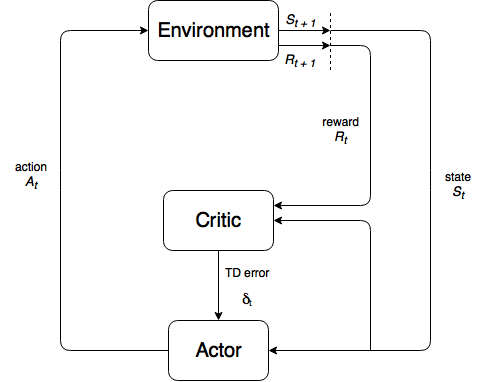
\includegraphics[scale = 0.5]{include/ActorCriticDiagram.png}
    \caption{A representation of the Actor-Critic model.
        The environment sends a state and reward signal to both the actor and the critic.
        The critic computes the TD-error, which the actor uses as an evaluation of its performance
        and then picks a new action and so forth.}
    \label{fig:actor-critic}
\end{figure}
%An advantage of using Actor-Critic methods is that the split into a actor and critic, reduces the variance of the function approximation, because the update step size for the policy parameters is defined relative to estimated value from critic.\cite{actCrit}


\subsubsection{Applying eligibility traces to the Actor-Critic method}\label{sec:actor_critic_el}

To increase the stability of the Actor-Critic method, we can extend it to use eligibility traces
for the weights of the policy and value estimators.
As described in section \ref{sec:et}, eligibility traces can be seen as the weighted trend
of the most recent gradient updates, and they can be updated as
\begin{equation}
    \mathbf{e}^{\theta} = \lambda \mathbf{e}^{\theta} + \nabla_\theta \log\pi(a|s,\theta_t)
\end{equation}
and
\begin{equation}
    \mathbf{e}^{\mathbf{w}} = \lambda \mathbf{e}^{\mathbf{w}} + \nabla_\mathbf{w} \hat{v}(s, \mathbf{w}_t)
\end{equation}

Using eligibility traces allows us to update the weights
according to the most recent trend of the gradients.
This has a stabilizing effect since it handles the problem of delayed reward.
I.e in most Atari games performing an action doesn't immediately return a reward,
which means that the wrong actions might be reinforced due to the illusion
of those actions being responsible for the gained reward.
The eligibility traces make sure that the change in weights is based on the
tendency of the gradients, and thus the actions that are responsible
for the earned reward also influence in the weight update.
In section \ref{sec:et} the weight update of the value estimator
using an eligibility trace was presented as the trace weighted by
the one-step TD-error.
To gain more control of the gradient steps, the step-size parameters $\alpha$ and $\beta$ are used,
as a mean to avoid traversing too far in the direction of the gradient.
\begin{equation*}
    \mathbf{w}_{t+1}= \mathbf{w}_t + \alpha \delta \mathbf{e}^{\mathbf{w}}
\end{equation*}
Equivalently the weights of the policy estimator can be updated in the same fashion
\begin{equation}
    \theta_{t+1} = \theta_t + \beta \delta \mathbf{e}^\theta
\end{equation}


%\printbibliography
%\bibliography{citations}
%\bibliographystyle{plain}
\end{document}
